%%
%% This is file `sample-acmsmall-conf.tex',
%% generated with the docstrip utility.
%%
%% The original source files were:
%%
%% samples.dtx  (with options: `acmsmall-conf')
%% 
%% IMPORTANT NOTICE:
%% 
%% For the copyright see the source file.
%% 
%% Any modified versions of this file must be renamed
%% with new filenames distinct from sample-acmsmall-conf.tex.
%% 
%% For distribution of the original source see the terms
%% for copying and modification in the file samples.dtx.
%% 
%% This generated file may be distributed as long as the
%% original source files, as listed above, are part of the
%% same distribution. (The sources need not necessarily be
%% in the same archive or directory.)
%%
%%
%% Commands for TeXCount
%TC:macro \cite [option:text,text]
%TC:macro \citep [option:text,text]
%TC:macro \citet [option:text,text]
%TC:envir table 0 1
%TC:envir table* 0 1
%TC:envir tabular [ignore] word
%TC:envir displaymath 0 word
%TC:envir math 0 word
%TC:envir comment 0 0
%%
%%
%% The first command in your LaTeX source must be the \documentclass command.
\documentclass[acmsmall]{acmart}
\usepackage[UTF8, fontset=macnew]{ctex}

%%
%% \BibTeX command to typeset BibTeX logo in the docs


%%
%% Submission ID.
%% Use this when submitting an article to a sponsored event. You'll
%% receive a unique submission ID from the organizers
%% of the event, and this ID should be used as the parameter to this command.
%%\acmSubmissionID{123-A56-BU3}

%%
%% The majority of ACM publications use numbered citations and
%% references.  The command \citestyle{authoryear} switches to the
%% "author year" style.
%%
%% If you are preparing content for an event
%% sponsored by ACM SIGGRAPH, you must use the "author year" style of
%% citations and references.
%% Uncommenting
%% the next command will enable that style.
%%\citestyle{acmauthoryear}

%%
%% end of the preamble, start of the body of the document source.
\begin{document}

%%
%% The "title" command has an optional parameter,
%% allowing the author to define a "short title" to be used in page headers.
% \title{Learn How to write a apporpriate resume by example - The preliminary text mining on the open data}
\title{透過實際案例學習如何撰寫好的求職履歷 - 使用文字探勘技術之初步研究}

%%
%% The "author" command and its associated commands are used to define
%% the authors and their affiliations.
%% Of note is the shared affiliation of the first two authors, and the
%% "authornote" and "authornotemark" commands
%% used to denote shared contribution to the research.

\author{李昀潔}
\affiliation{%
    \institution{資管博一}
}
\author{呂孟芸}
\affiliation{%
    \institution{國企大四}
}
\author{張譯心}
\affiliation{%
    \institution{國企大四}
}
\author{陳韋霖}
\affiliation{%
    \institution{資工碩一}
}
\author{詹雅安}
\affiliation{%
    \institution{會計大四}
}

%%
%% By default, the full list of authors will be used in the page
%% headers. Often, this list is too long, and will overlap
%% other information printed in the page headers. This command allows
%% the author to define a more concise list
%% of authors' names for this purpose.
% \renewcommand{\shortauthors}{Trovato and Tobin, et al.}

%%
%% The abstract is a short summary of the work to be presented in the
%% article.
\begin{abstract}
    對於學生而言,除了努力完成學業或完成研究以取得畢業之外,
    如何透過簡歷(Resume)的撰寫去應徵企業的招募也是一件重要的事。
    然而如何撰寫簡歷不是一件簡單的。
    因此我們小組從網際網路上找尋到一個人簡歷的開放資料集,
    透過分群方法(Clustering)來對該資料集進行研究,
    我們檢驗履歷的寫法是否能對應到公司招聘的職位,
    另外我們也找出一些能夠申請多種工作類別的簡歷寫法,
    此次研究希望透過該開放資料集所作的初步研究,
    希望能對學生們製作個人簡歷上能有所幫助。
\end{abstract}

%%
%% The code below is generated by the tool at http://dl.acm.org/ccs.cfm.
%% Please copy and paste the code instead of the example below.
%%

\begin{CCSXML}
<ccs2012>
   <concept>
       <concept_id>10010405</concept_id>
       <concept_desc>Applied computing</concept_desc>
       <concept_significance>500</concept_significance>
       </concept>
   <concept>
       <concept_id>10010405.10010497</concept_id>
       <concept_desc>Applied computing~Document management and text processing</concept_desc>
       <concept_significance>500</concept_significance>
       </concept>
 </ccs2012>
\end{CCSXML}

\ccsdesc[500]{Applied computing}
\ccsdesc[500]{Applied computing~Document management and text processing}

\ccsdesc[500]{Applied computing}


%%
%% Keywords. The author(s) should pick words that accurately describe
%% the work being presented. Separate the keywords with commas.
% \keywords{datasets, neural networks, gaze detection, text tagging}

%% A "teaser" image appears between the author and affiliation
%% information and the body of the document, and typically spans the
%% page.
\iffalse
\begin{teaserfigure}
  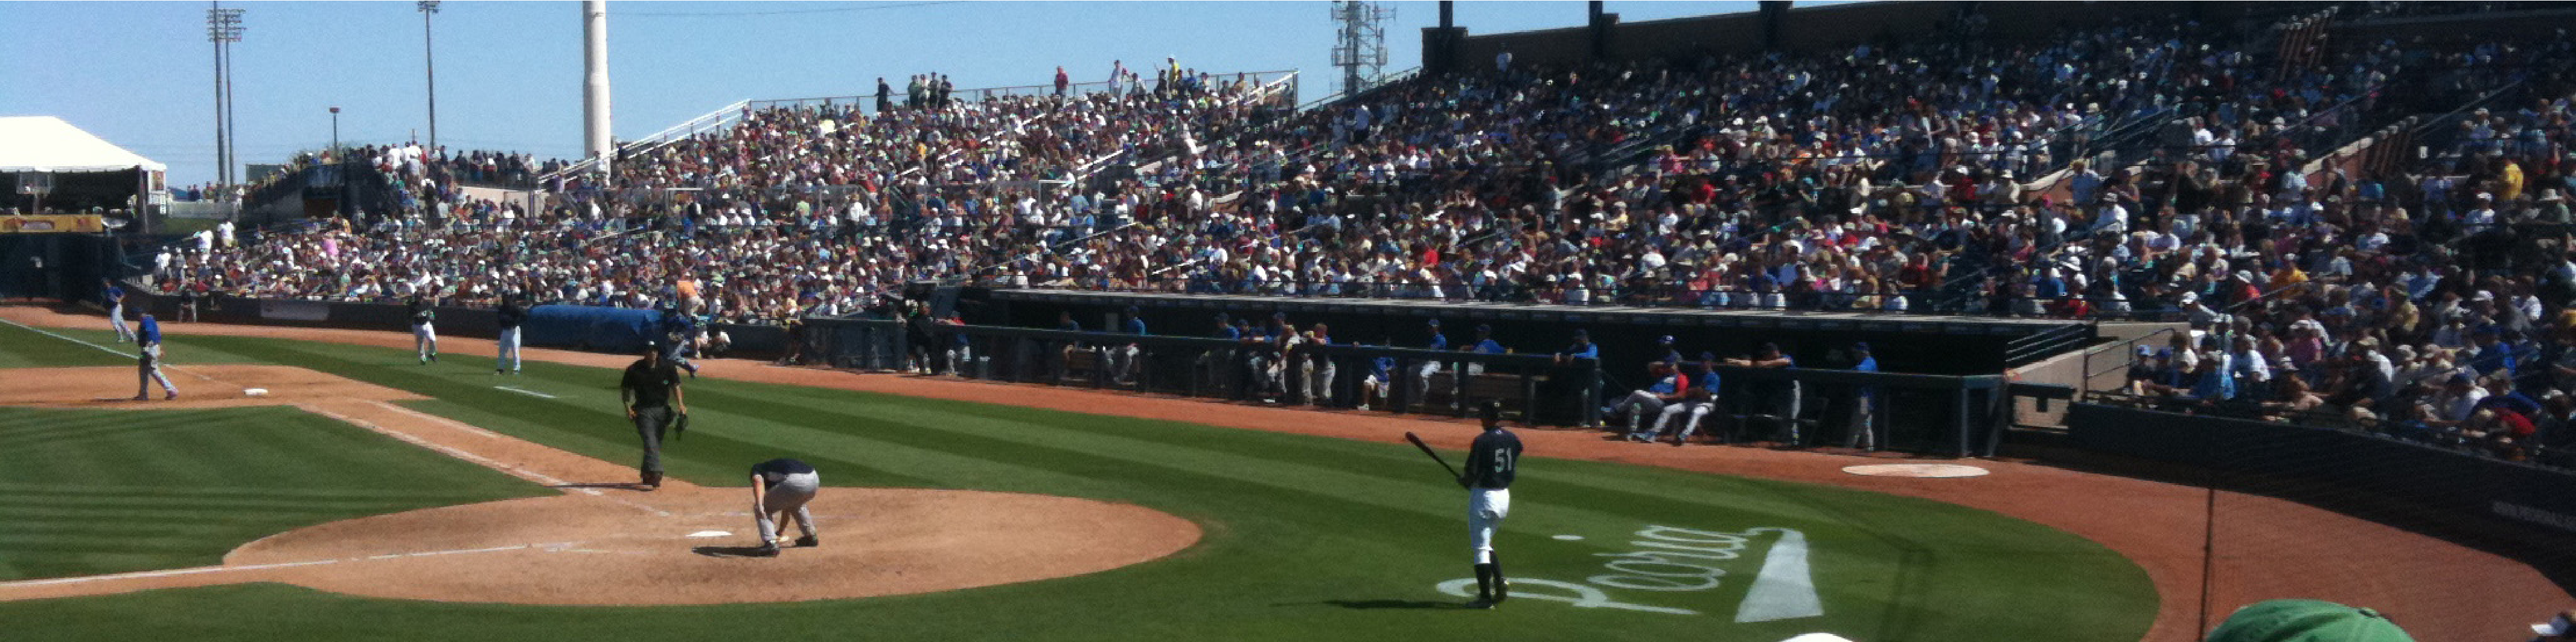
\includegraphics[width=\textwidth]{sampleteaser}
  \caption{Seattle Mariners at Spring Training, 2010.}
  \Description{Enjoying the baseball game from the third-base
  seats. Ichiro Suzuki preparing to bat.}
  \label{fig:teaser}
\end{teaserfigure}
\fi

%%
%% This command processes the author and affiliation and title
%% information and builds the first part of the formatted document.
\maketitle

\section{研究目標}

投履歷找工作時,
如何撰寫一份符合業主要求的履歷,
尤其對於高度專業的工作而言,
更顯重要,
然此環節雖坊間有許多教條方法供大眾學習,


\section{研究方法}

\subsection{分群方法}

\section{實驗結果}

\subsection{簡歷一致性}

\subsection{跨領域範本}

\section{結論}

% \section{Template Overview}
% \subsection{Template Styles}


%%
%% The acknowledgments section is defined using the "acks" environment
%% (and NOT an unnumbered section). This ensures the proper
%% identification of the section in the article metadata, and the
%% consistent spelling of the heading.
\begin{acks}
    謝謝老師的教導,使得我們能得以完成此次報告研究。
\end{acks}

%%
%% The next two lines define the bibliography style to be used, and
%% the bibliography file.
\bibliographystyle{ACM-Reference-Format}
\bibliography{sample-base}

\end{document}
\endinput
%%
%% End of file `sample-acmsmall-conf.tex'.
